\documentclass{beamer}\usepackage[]{graphicx}\usepackage[]{xcolor}
% maxwidth is the original width if it is less than linewidth
% otherwise use linewidth (to make sure the graphics do not exceed the margin)
\makeatletter
\def\maxwidth{ %
  \ifdim\Gin@nat@width>\linewidth
    \linewidth
  \else
    \Gin@nat@width
  \fi
}
\makeatother

\definecolor{fgcolor}{rgb}{0.345, 0.345, 0.345}
\newcommand{\hlnum}[1]{\textcolor[rgb]{0.686,0.059,0.569}{#1}}%
\newcommand{\hlstr}[1]{\textcolor[rgb]{0.192,0.494,0.8}{#1}}%
\newcommand{\hlcom}[1]{\textcolor[rgb]{0.678,0.584,0.686}{\textit{#1}}}%
\newcommand{\hlopt}[1]{\textcolor[rgb]{0,0,0}{#1}}%
\newcommand{\hlstd}[1]{\textcolor[rgb]{0.345,0.345,0.345}{#1}}%
\newcommand{\hlkwa}[1]{\textcolor[rgb]{0.161,0.373,0.58}{\textbf{#1}}}%
\newcommand{\hlkwb}[1]{\textcolor[rgb]{0.69,0.353,0.396}{#1}}%
\newcommand{\hlkwc}[1]{\textcolor[rgb]{0.333,0.667,0.333}{#1}}%
\newcommand{\hlkwd}[1]{\textcolor[rgb]{0.737,0.353,0.396}{\textbf{#1}}}%
\let\hlipl\hlkwb

\usepackage{framed}
\makeatletter
\newenvironment{kframe}{%
 \def\at@end@of@kframe{}%
 \ifinner\ifhmode%
  \def\at@end@of@kframe{\end{minipage}}%
  \begin{minipage}{\columnwidth}%
 \fi\fi%
 \def\FrameCommand##1{\hskip\@totalleftmargin \hskip-\fboxsep
 \colorbox{shadecolor}{##1}\hskip-\fboxsep
     % There is no \\@totalrightmargin, so:
     \hskip-\linewidth \hskip-\@totalleftmargin \hskip\columnwidth}%
 \MakeFramed {\advance\hsize-\width
   \@totalleftmargin\z@ \linewidth\hsize
   \@setminipage}}%
 {\par\unskip\endMakeFramed%
 \at@end@of@kframe}
\makeatother

\definecolor{shadecolor}{rgb}{.97, .97, .97}
\definecolor{messagecolor}{rgb}{0, 0, 0}
\definecolor{warningcolor}{rgb}{1, 0, 1}
\definecolor{errorcolor}{rgb}{1, 0, 0}
\newenvironment{knitrout}{}{} % an empty environment to be redefined in TeX

\usepackage{alltt}
\usetheme{Boadilla}

\makeatother
\setbeamertemplate{footline}
{
    \leavevmode%
    \hbox{%
    \begin{beamercolorbox}[wd=.4\paperwidth,ht=2.25ex,dp=1ex,center]{author in head/foot}%
        \usebeamerfont{author in head/foot}\insertshortauthor
    \end{beamercolorbox}%
    \begin{beamercolorbox}[wd=.55\paperwidth,ht=2.25ex,dp=1ex,center]{title in head/foot}%
        \usebeamerfont{title in head/foot}\insertshorttitle
    \end{beamercolorbox}%
    \begin{beamercolorbox}[wd=.05\paperwidth,ht=2.25ex,dp=1ex,center]{date in head/foot}%
        \insertframenumber{}
    \end{beamercolorbox}}%
    \vskip0pt%
}
\makeatletter
\setbeamertemplate{navigation symbols}{}

\usepackage[T1]{fontenc}
\usepackage{lmodern}
\usepackage{amssymb,amsmath,bm,bbm}
\renewcommand{\familydefault}{\sfdefault}

\usepackage{mathtools}
\usepackage{graphicx}
\usepackage{threeparttable}
\usepackage{booktabs}
\usepackage{siunitx}
\sisetup{parse-numbers=false}

\setlength{\OuterFrameSep}{-2pt}
\makeatletter
\preto{\@verbatim}{\topsep=-10pt \partopsep=-10pt }
\makeatother

\title[Week 3:\ Random Utility Model]{Week 3:\ Random Utility Model}
\author[ResEcon 703:\ Advanced Econometrics]{ResEcon 703:\ Topics in Advanced Econometrics}
\date{Matt Woerman\\University of Massachusetts Amherst}
\IfFileExists{upquote.sty}{\usepackage{upquote}}{}
\begin{document}


{\setbeamertemplate{footline}{} 
\begin{frame}[noframenumbering]
    \titlepage
\end{frame}
}

\begin{frame}\frametitle{Agenda}
    Last two weeks
    \begin{itemize}
    	\item Structural estimation
      \item R tutorial
    \end{itemize}
    \vspace{2ex}
    This week's topics
    \begin{itemize}
    	\item \hyperlink{page.\getpagerefnumber{dc}}{Discrete choice}
        \item \hyperlink{page.\getpagerefnumber{rum}}{Random utility model}
        \item \hyperlink{page.\getpagerefnumber{probabilities}}{Choice probabilities}
        \item \hyperlink{page.\getpagerefnumber{lpm}}{Linear probability model}
        \item \hyperlink{page.\getpagerefnumber{example}}{Linear probability model R example}
    \end{itemize}
    \vspace{2ex}
    This week's reading
    \begin{itemize}
        \item Train textbook, chapters 1--2
    \end{itemize}
\end{frame}

\section{Discrete Choice}
\label{dc}
\begin{frame}\frametitle{}
    \vfill
    \centering
    \begin{beamercolorbox}[center]{title}
        \Large Discrete Choice
    \end{beamercolorbox}
    \vfill
\end{frame}

\begin{frame}\frametitle{How to Construct a Structural Econometric Model}
	\begin{enumerate}
		\item Start with economic theory
		\item Transform economic model into econometric model
		\item Estimate the econometric model
	\end{enumerate}
	\vspace{3ex}
	We will use a consistent framework for the first 1.5 steps
	\begin{itemize}
		\item Step 1: Discrete choice to maximize utility
		\item Step 2a: Random utility model
		\item (Step 2b: We will make different assumptions about the unobservables in the random utility model, yielding different econometric models)
	\end{itemize}
\end{frame}

\begin{frame}\frametitle{Discrete Choice}
    Many problems in microeconomics and related fields involve a decision maker choosing between a discrete set of alternatives
    \begin{itemize}	
    	\item Which travel mode a commuter uses to get to work
    	\item Which health insurance plan an employee chooses
    	\item Which recreation site to visit
    	\item What consumer goods a household purchases
    	\item Which job a worker chooses
    	\item Which city a household chooses to locate in
    	\item What pollution control equipment a power plant installs
    	\item Whether a city replaces a bus engine
    	\item Which automobile a household purchases
    	\item Which crop a farmer plants
    \end{itemize}
\end{frame}

\begin{frame}\frametitle{Analyzing a Discrete Choice Problem}
    Three steps to set up and analyze a discrete choice problem
    \begin{enumerate}
    	\item Specify the choice set
    	\item Formulate a model of how the agent chooses among the choice set
    	\item Estimate the unknown parameters of the model
    	\begin{itemize}
    		\item These are the structural parameters that describe the decision maker's behavior, preferences, etc.
    	\end{itemize}
    \end{enumerate}
\end{frame}

\begin{frame}\frametitle{Choice Set}
    The choice set defines all of the possible alternatives available to the decision maker
    \begin{itemize}
    	\item Example: How to get to campus?
    	\begin{itemize}
    		\item Drive alone, carpool, bus, bike, walk, Uber, stay home, etc.
    	\end{itemize}
    \end{itemize}
    \vspace{2ex}
    Alternatives must be mutually exclusive and exhaustive
    \begin{itemize}
    	\item Mutually exclusive: The agent may choose only one alternative, and choosing that alternative precludes choosing any other alternative
    	\item Exhaustive: That agent must chooses one of the alternatives, so all possible alternatives must be included
    \end{itemize}
    \vspace{2ex}
    The choice set will depend on the context, research question, data availability, etc.
\end{frame}

\begin{frame}\frametitle{Discrete Choice Model and Estimation}
    Step 2: Formulate a model of how the agent chooses among the choice set \\
    \begin{itemize}
    	\item Random utility model
    	\begin{itemize}
    		\item The general model is coming up next
    		\item We will talk about a few specific models throughout the semester
    	\end{itemize}
    \end{itemize}
    \vspace{3ex}
    Step 3: Estimate the unknown parameters on the model
    \begin{itemize}
    	\item Estimation methods: the rest of the semester
    \end{itemize}
\end{frame}

\section{Random Utility Model}
\label{rum}
\begin{frame}\frametitle{}
    \vfill
    \centering
    \begin{beamercolorbox}[center]{title}
        \Large Random Utility Model
    \end{beamercolorbox}
    \vfill
\end{frame}

\begin{frame}\frametitle{Random Utility Model}
    Discrete choices are usually modeled under the assumption of utility-maximizing behavior by the decision maker (or profit maximization when the decision maker is a firm) \\
    \vspace{2ex} 
    The random utility model (RUM) provides such a framework
    \begin{itemize}
    	\item The agent gets some amount of utility from each of the alternatives
    	\begin{itemize}
    		\item The amount of utility can depend on observed characteristics of the alternatives, observed characteristics of the decision maker, and unobserved characteristics
    	\end{itemize}
    	\item The agent selects the alternative that provides the greatest utility
    \end{itemize}
    \vspace{2ex}
    Models derived from RUM are consistent with utility (or profit) maximization, even if the decision maker does not maximize utility
    \begin{itemize}
    	\item RUMs can be highly flexible and include behavioral and information parameters that diverge from the traditional neoclassical model
    \end{itemize}
\end{frame}

\begin{frame}\frametitle{Specifying a Random Utility Model}
	The model from the perspective of the decision maker
	\begin{itemize}
		\item A decision maker, $n$, faces a choice among $J$ alternatives
    	\item Alternative $j$ provides utility $U_{nj}$ (where $j = 1, \ldots, J$)
    	\item The decision maker chooses the alternative with the greatest utility
    	\begin{itemize}
    		\item $n$ chooses $i$ if and only if $U_{ni} > U_{nj} \; \forall j \neq i$
    	\end{itemize}
   	\end{itemize}
   	\vspace{3ex}
   	But we (the econometricians) do not observe $U_{nj}$!
   	\begin{itemize}
   		\item We observe
   		\begin{itemize}
   			\item The chosen alternative
   			\item Some attributes of each alternative
   			\item Some attributes of the decision maker
   		\end{itemize}
   		\item We will use these data to infer $U_{nj}$ and how each attribute affects $U_{nj}$
   	\end{itemize}
\end{frame}

\begin{frame}\frametitle{Model of Utility}
	Decompose the utility of each alternative, $U_{nj}$, into two components
	\begin{itemize}
		\item Utility of observed factors: $V_{nj}$
		\item Utility of unobserved factors: $\varepsilon_{nj}$
	\end{itemize}
	$$U_{nj} = V_{nj} + \varepsilon_{nj}$$ \\
	\vspace{2ex}
	$V_{nj} = V(\bm{x}_{nj}, \bm{s}_n)$ is called representative utility
	\begin{itemize}
		\item $\bm{x}_{nj}$: Vector of attributes of the alternative
		\item $\bm{s}_n$: Vector of attributes of the decision maker
	\end{itemize}
	\vspace{2ex}
	$\varepsilon_{nj}$ is everything that affects utility not included in $V_{nj}$
	\begin{itemize}
		\item Depends importantly on the specification of $V_{nj}$
		\item We treat this term as a random variable from our perspective
		\item $f(\bm{\varepsilon}_n)$ is the joint density of the random vector $\bm{\varepsilon}_n = \{\varepsilon_{n1}, \dots, \varepsilon_{nJ}\}$ for decision maker $n$
	\end{itemize}
\end{frame}

\begin{frame}\frametitle{Representative Utility}
  We model representative utility, $V_{nj}$, as a function of
  \begin{itemize}
		\item $\bm{x}_{nj}$: Vector of attributes of the alternative
		\item $\bm{s}_n$: Vector of attributes of the decision maker
		\item $\bm{\beta}$: Vector of structural parameters
	\end{itemize}
	\vspace{2ex}
	We usually specify representative utility as a linear function
    $$V_{nj} = \bm{\beta}' \bm{x}_{nj}$$ \\
    \begin{itemize}
    	\item A linear function is highly flexible and can include interactions, squared terms, etc.
    	\item Most utility functions can be closely approximated by a function that is linear in parameters
    	\item Non-linear utility can greatly complicate estimation
    \end{itemize}
\end{frame}

\begin{frame}\frametitle{Structural Parameters}
  With linear representative utility, the total utility that alternative $j$ gives decision maker $n$ is
  $$U_{nj} = \bm{\beta}' \bm{x}_{nj} + \varepsilon_{nj}$$ \\
  \vspace{2ex}
  The structural parameters, $\bm{\beta}$, tell us how the observable attributes relate to the unobserved utility
  \begin{itemize}
    \item With linear representative utility, these parameters are interpreted as marginal utilities
    \item We can recover other structural parameters with different models of utility, profit, etc.
  \end{itemize}
  \vspace{2ex}
  We want to find the structural parameters that make these utilities consistent with the observed choices
  \begin{itemize}
    \item More on how to do this for the rest of the semester
  \end{itemize}
\end{frame}

\section{Choice Probabilities}
\label{probabilities}
\begin{frame}\frametitle{}
    \vfill
    \centering
    \begin{beamercolorbox}[center]{title}
        \Large Choice Probabilities
    \end{beamercolorbox}
    \vfill
\end{frame}

\begin{frame}\frametitle{Choice Probabilities}
  If you knew the representative utility, $V_{nj}$, for every alternative, could you say for certain what the decision maker would choose?
  \begin{itemize}
    \item No!
  \end{itemize}
  \vspace{2ex}
	We assume the decision maker chooses the alternative that maximizes total utility, not representative utility
	\begin{itemize}
	  \item We model utility as containing an unobserved random component
		\item Knowing representative utility is not sufficient to make a definitive statement about which alternative maximizes utility
	\end{itemize}
	\vspace{2ex}
	If we cannot model discrete choices with certainty, what can we do?
	\begin{itemize}
		\item We can make probabilistic statements!
	\end{itemize}
	\vspace{2ex}
	Choice probabilities play an important role in discrete choice models
	\begin{itemize}
		\item Probability of the decision maker choosing each of the alternatives
	\end{itemize}
\end{frame}

\begin{frame}\frametitle{General Formula for Choice Probabilities}
    The probability that decision maker $n$ chooses alternative $i$ is
    \begin{align*}
    	P_{ni} & = \Pr(U_{ni} > U_{nj} \; \forall j \neq i) \\
    	& = \Pr(V_{ni} + \varepsilon_{ni} > V_{nj} + \varepsilon_{nj} \; \forall j \neq i) \\
    	& = \Pr(\varepsilon_{nj} - \varepsilon_{ni} < V_{ni} - V_{nj} \; \forall j \neq i) \\
    	& = \int_{\bm{\varepsilon}} \mathbbm{1}(\varepsilon_{nj} - \varepsilon_{ni} < V_{ni} - V_{nj} \; \forall j \neq i) f(\bm{\varepsilon}_n) d\bm{\varepsilon}_n
    \end{align*} \\
    \vspace{2ex}
    This probability is the cumulative distribution of $\varepsilon_{nj} - \varepsilon_{ni}$
    \begin{itemize}
    	\item Multidimensional integral over the density of the unobserved component of utility, $f(\bm{\varepsilon}_n)$
    	\item Assumptions about $f(\bm{\varepsilon}_n)$ yield different discrete choice models
    \end{itemize}
\end{frame}

\begin{frame}\frametitle{Choice Probabilities Example}
    A person chooses whether to take a car ($c$) or a bus ($b$) to work
    \begin{itemize}
    	\item We observe the time, $T$, and cost, $M$, of each alternative
    \end{itemize}
    \vspace{1ex}
    We specify the representative utility of each alternative as
    \begin{align*}
    	V_{nc} & = \beta_{0c} + \beta_1 T_{nc} + \beta_2 M_{nc} \\
    	V_{nb} & = \beta_{0b} + \beta_1 T_{nb} + \beta_2 M_{nb}
    \end{align*}
    Suppose the $\beta$ coefficients are known 
    \begin{itemize}
    	\item Then $V_{nc}$ and $V_{nb}$ are known, so we know which travel mode has greater representative utility
    	\item But unobserved factors also affect this decision: $\varepsilon_{nc}$ and $\varepsilon_{nb}$
    \end{itemize}
    \vspace{1ex}
    The choice probability of driving is
    \begin{align*}
    	P_{nc} & = \Pr(\varepsilon_{nb} - \varepsilon_{nc} < V_{nc} - V_{nb}) \\
    	& = \Pr(\varepsilon_{nb} - \varepsilon_{nc} < (\beta_{0c} + \beta_1 T_{nc} + \beta_2 M_{nc}) - (\beta_{0b} + \beta_1 T_{nb} + \beta_2 M_{nb})) \\
    	& = \Pr(\varepsilon_{nb} - \varepsilon_{nc} < (\beta_{0c} - \beta_{ob}) + \beta_1(T_{nc} - T_{nb}) + \beta_2(M_{nc} - M_{nb}))
    \end{align*}
\end{frame}

\begin{frame}\frametitle{Using Choice Probabilities To Estimate Parameters}    
	We want to estimate the structural parameters of the model that describe the decision maker's preferences, behavior, etc.
	\begin{itemize}
		\item How do these choice probabilities help us with that?
	\end{itemize}
	\vspace{2ex}
	We want to fit the model to the data, but what makes for a good fit?
	\begin{itemize}
		\item When decision maker $n$ chooses alternative $i$, we want that choice probability, $P_{ni}$, to be close to $1$
		\item And we want all other choice probabilities to be close to $0$
		\item So ``fitting the model'' means finding the structural parameters that fit the choice probabilities to the observed choices
	\end{itemize}
	\vspace{2ex}
	How we do that will depend on the assumptions we make about $f(\bm{\varepsilon}_n)$
	\begin{itemize}
		\item More on that starting next week
	\end{itemize}
\end{frame}

\begin{frame}\frametitle{Properties of the Random Utility Model}
	$$P_{ni} = \int_{\bm{\varepsilon}} \mathbbm{1}(\varepsilon_{nj} - \varepsilon_{ni} < V_{ni} - V_{nj} \; \forall j \neq i) f(\bm{\varepsilon}_n) d\bm{\varepsilon}_n$$ \\
	\vspace{2ex}
    The general formula for choice probabilities reveals two important properties about the random utility model
    \begin{itemize}
    	\item Only difference in utility matter
    	\begin{itemize}
    		\item We ultimately do not care about the level of utility from any alternative, just the comparisons between any two alternatives
    		\item We can only estimate parameters that capture differences between alternatives
    	\end{itemize}
    	\item The scale of utility is arbitrary
    	\begin{itemize}
    		\item Scaling all utilities does not change the comparison between alternatives
    		\item We will usually normalize the variance of the error terms 
    	\end{itemize}
    \end{itemize}
    \vspace{2ex}
    We will talk about these properties more when we talk about estimation
\end{frame}

\section{Linear Probability Model}
\label{lpm}
\begin{frame}\frametitle{}
    \vfill
    \centering
    \begin{beamercolorbox}[center]{title}
        \Large Linear Probability Model
    \end{beamercolorbox}
    \vfill
\end{frame}

\begin{frame}\frametitle{Binary Choice}
    The discrete choice problem is greatly simplified with only two alternatives
    \begin{itemize}
    	\item With only two alternatives, there is only one comparison to model
    \end{itemize}
    \vspace{3ex}
    The choice probabilities can be fully described with only one equation 
    $$P_{n1} = \Pr(\varepsilon_{n2} - \varepsilon_{n1} < V_{n1} - V_{n2})$$ \\
    \begin{itemize}
    	\item If the choice set is mutually exclusive and exhaustive, then it must be the case that $P_{n2} = 1 - P_{n1}$
    \end{itemize}
    \vspace{3ex}
    We will typically assume representative utility is linear: $V_{ni} = \bm{\beta}' \bm{x}_{ni}$
    $$P_{n1} = \Pr(\varepsilon_{n2} - \varepsilon_{n1} < \bm{\beta}' (\bm{x}_{n1} - \bm{x}_{n2}))$$
\end{frame}

\begin{frame}\frametitle{Linear Probability Model}
    Abstract from our structural model for the rest of this lecture and consider a nonstructural approach to estimate a binary choice model
    \begin{itemize}
    	\item We will return to structural estimation next week and for the remainder of the course
    \end{itemize}
    \vspace{2ex}
	From the structural model, the choice probability $P_{n1}$ is a nonlinear function of data about each alternative, $\bm{x}_n = \{\bm{x}_{n1}, \bm{x}_{n2}\}$
	\begin{itemize}
	  \item A simple linear analog of this choice probability is
    $$Y_n = \bm{\alpha}' \bm{x}_n + \omega_n$$
    where $Y_n = 1$ if and only if $n$ chooses alternative $1$
	\end{itemize}
    \vspace{2ex}
    Under standard OLS assumptions
    $$\Pr(Y_n = 1 \mid \bm{x}_n) = E(Y_n \mid \bm{x}_n) = \bm{\alpha}' \bm{x}_n$$
    So this OLS regression model is called the linear probability model (LPM)
\end{frame}

\begin{frame}\frametitle{Linear Probability Model Example}
    A person chooses whether to take a car ($c$) or a bus ($b$) to work
    \begin{itemize}
    	\item We observe the time, $T$, and cost, $M$, of each choice
    \end{itemize}
    \vspace{2ex}
    The choice probability of driving is
    \begin{align*}
    	P_{nc} & = \Pr(\varepsilon_{nb} - \varepsilon_{nc} < V_{nc} - V_{nb}) \\
    	& = \Pr(\varepsilon_{nb} - \varepsilon_{nc} < (\beta_{oc} + \beta_1 T_{nc} + \beta_2 M_{nc}) - (\beta_{0b} + \beta_1 T_{nb} + \beta_2 M_{nb})) \\
    	& = \Pr(\varepsilon_{nb} - \varepsilon_{nc} < (\beta_{0c} - \beta_{ob}) + \beta_1(T_{nc} - T_{nb}) + \beta_2(M_{nc} - M_{nb}))
    \end{align*} \\
    \vspace{2ex}
    A nonstructural approach to estimate this choice is to use OLS to estimate the linear probability model
    $$Y_n = \alpha_0 + \alpha_1 T_{nc} + \alpha_2 T_{nb} + \alpha_3 M_{nc} + \alpha_4 M_{nb} + \omega_n$$
    where $Y_n = 1$ if and only if $n$ chooses to drive
\end{frame}

\begin{frame}\frametitle{Pros and Cons of the Linear Probability Model}
    Pros
    \begin{itemize}
    	\item You can estimate the LPM using OLS
    	\begin{itemize}
    		\item Regression is fast and easy to run
    		\item Assumptions are transparent and well-known
    	\end{itemize}
    	\item Coefficients can be interpreted as marginal effects
    \end{itemize}
    \vspace{2ex}
    Cons
    \begin{itemize}
    	\item Probabilities are not bounded by $[0, 1]$
    	\begin{itemize}
    		\item Coefficients can be biased and inconsistent
    	\end{itemize}
    	\item Coefficients are not structural parameters
    	\begin{itemize}
    		\item Marginal effects are generally not the same thing as marginal utility or any other parameter that defines preferences, behavior, etc.
    	\end{itemize}
    	\item Error terms are heteroskedastic and not normally distributed
    \end{itemize}
    \vspace{2ex}
    Whether the pros outweigh the cons depends on your context, research question, data, etc.
\end{frame}

\begin{frame}\frametitle{Nonstructural Approach for Multinomial Choice}
    We can use OLS to nonstructurally estimate a linear probability model of a binary choice
    \begin{itemize}
    	\item It may or may not be the best method, but it is feasible and has some advantages
    \end{itemize}
    \vspace{3ex}
    What if you have a multinomial choice (more than two alternatives)?
    \begin{itemize}
    	\item Can you think of an OLS (or other nonstructural) approach to estimate all of the comparisons implicit in a multinomial choice?
    \end{itemize}
    \vspace{3ex}
    As we move to more complicated choice settings, a structural approach becomes the most feasible way to credibly estimate a model of discrete choice
\end{frame}

\section{Linear Probability Model R Example}
\label{example}
\begin{frame}\frametitle{}
    \vfill
    \centering
    \begin{beamercolorbox}[center]{title}
        \Large Linear Probability Model R Example
    \end{beamercolorbox}
    \vfill
\end{frame}

\begin{frame}\frametitle{Binary Choice Example}
    We are studying how consumers make choices about expensive and highly energy-consuming appliances in their homes.
    \begin{itemize}
        \item We have (simulated) data on 600 households that rent apartments without air conditioning. These households must choose whether or not to purchase a window air conditioning unit. (To simplify things, we assume there is only one ``representative'' air conditioner for each household and its price and operating cost are exogenous.)
        \item We observe the following data about each household and its ``representative'' air conditioner
        \begin{itemize}
            \item An indicator if they purchase the air conditioner (TRUE/FALSE)
            \item The purchase price of the air conditioner (\$)
            \item The annual operating cost of the air conditioner (\$ per year)
            \item The household's electricity price (cents per kWh)
            \item The size of the household's apartment (square feet)
            \item The household's annual income (\$1000s)
            \item The number of residents in the household (people)
            \item An indicator for the household's city (1, 2, or 3) 
        \end{itemize}
    \end{itemize}
\end{frame}

\begin{frame}\frametitle{Random Utility Model for Air Conditioner Choice}
    We model the utility to household $n$ of not purchasing an air conditioned ($j = 0$) or purchasing an air conditioner ($j = 1$) as
    \begin{align*}
        U_{n0} & = V_{n0} + \varepsilon_{n0} \\
        U_{n1} & = V_{n1} + \varepsilon_{n1}
    \end{align*}
    where $V_{nj}$ depends on the data about alternative $j$ and household $n$ \\
    \vspace{3ex}
    The probability that household $n$ purchases an air conditioner is
    $$P_{n1} = \Pr(\varepsilon_{n0} - \varepsilon_{n1} < V_{n1} - V_{n0})$$ \\
    \begin{itemize}
        \item Only differences in utility---not the actual values of utility---affect this probability
        \item What is the difference in utility to household $n$ from purchasing an air conditioner vs.\ not purchasing an air conditioner?
    \end{itemize}
\end{frame}

\begin{frame}\frametitle{Representative Utility for Air Conditioner Choice}
    \vspace{-2ex}
    $$P_{n1} = \Pr(\varepsilon_{n0} - \varepsilon_{n1} < V_{n1} - V_{n0})$$ \\
    \vspace{1ex}
    What is the difference in utility to household $n$ from purchasing an air conditioner vs.\ not purchasing an air conditioner?
    \begin{itemize}
        \item They gain utility from having air conditioning
        \item They lose utility from paying the purchase price of the air conditioner
        \item They lose utility from paying the annual operating cost of the air conditioner
    \end{itemize}
    \vspace{2ex}
    We can model the difference in utility as
    $$V_{n1} - V_{n0} = \beta_0 - \beta_1 P_n - \beta_2 C_n$$
    where
    \begin{itemize}
        \item $P_n$ is the purchase price of the air conditioner
        \item $C_n$ is the annual operating cost of the air conditioner
        \item $\beta_0$, $\beta_1$, and $\beta_2$ are utility parameters to be estimated
    \end{itemize}
\end{frame}

\begin{frame}\frametitle{Nonstructural Approach to Air Conditioner Choice}
    \vspace{-2ex}
    $$P_{n1} = \Pr(\varepsilon_{n0} - \varepsilon_{n1} < \beta_0 - \beta_1 P_n - \beta_2 C_n)$$ \\
    \vspace{1ex}
    Can we estimate the parameters of this model using an OLS regression?
    \begin{itemize}
        \item No, it is nonlinear
        \item But we can use this model to inform a nonstructural approach to estimation
    \end{itemize}
    \vspace{2ex}
    The probability that household $n$ purchases an air conditioner depends on:
    \begin{itemize}
        \item The price of the air conditioner
        \item The annual operating cost of the air conditioner
        \item Some parameters
        \item Random errors
    \end{itemize}
    \vspace{2ex}
    We can construct a linear probability model with all of these characteristics
\end{frame}

\begin{frame}\frametitle{Linear Probability Model for Air Conditioner Choice}
    We can use a linear probability model to see how the purchase price and the operating cost affect the decision to purchase.
    $$Y_n = \alpha_0 + \alpha_1 P_n + \alpha_2 C_n + \omega_n$$
    where
    \begin{itemize}
        \item $Y_n = 1$ if and only if $n$ purchases an air conditioner
        \item $P_n$ is the purchase price of the air conditioner
        \item $C_n$ is the annual operating cost of the air conditioner
    \end{itemize}
    \vspace{3ex}
    Note that this regression model is not the same as our structural model!
    $$P_{n1} = \Pr(\varepsilon_{n0} - \varepsilon_{n1} < \beta_0 - \beta_1 P_n - \beta_2 C_n)$$ \\
    \begin{itemize}
        \item But the choice probability from the structural model has informed what should go in our nonstructural OLS regression
    \end{itemize}
\end{frame}

\begin{frame}[fragile]\frametitle{Load Dataset}
    \texttt{read\_csv()} is a \texttt{tidyverse} function to read a .csv file into a tibble
\begin{knitrout}\footnotesize
\definecolor{shadecolor}{rgb}{0.969, 0.969, 0.969}\color{fgcolor}\begin{kframe}
\begin{alltt}
\hlcom{## Load tidyverse}
\hlkwd{library}\hlstd{(tidyverse)}
\end{alltt}
\end{kframe}
\end{knitrout}
\begin{knitrout}\footnotesize
\definecolor{shadecolor}{rgb}{0.969, 0.969, 0.969}\color{fgcolor}\begin{kframe}
\begin{alltt}
\hlcom{## Load dataset}
\hlstd{ac_data} \hlkwb{<-} \hlkwd{read_csv}\hlstd{(}\hlstr{'ac_renters.csv'}\hlstd{)}
\end{alltt}


{\ttfamily\noindent\itshape\color{messagecolor}{\#\# Rows: 600 Columns: 8\\\#\# -- Column specification ----------------------------------------------\\\#\# Delimiter: "{},"{}\\\#\# dbl (7): cost\_system, cost\_operating, elec\_price, square\_feet, inc...\\\#\# lgl (1): air\_conditioning\\\#\# \\\#\# i Use `spec()` to retrieve the full column specification for this data.\\\#\# i Specify the column types or set `show\_col\_types = FALSE` to quiet this message.}}\end{kframe}
\end{knitrout}
\end{frame}

\begin{frame}[fragile]\frametitle{Dataset}
\begin{knitrout}\footnotesize
\definecolor{shadecolor}{rgb}{0.969, 0.969, 0.969}\color{fgcolor}\begin{kframe}
\begin{alltt}
\hlcom{## Look at dataset}
\hlstd{ac_data}
\end{alltt}
\begin{verbatim}
## # A tibble: 600 x 8
##    air_conditio~1 cost_~2 cost_~3 elec_~4 squar~5 income resid~6  city
##    <lgl>            <dbl>   <dbl>   <dbl>   <dbl>  <dbl>   <dbl> <dbl>
##  1 FALSE              513     247    12.8     541     47       2     1
##  2 FALSE              578     138     9.6     384     64       1     1
##  3 TRUE               658     171    10.7     619     86       2     1
##  4 FALSE              615     198    11.5     624     49       2     1
##  5 FALSE              515     165    10.5     365     56       1     1
##  6 FALSE              588     143     9.7     411     39       2     1
##  7 TRUE               643     153    10.1     529     58       2     1
##  8 FALSE              676     182    11       694     46       2     1
##  9 TRUE               516     137     9.6     305     75       1     1
## 10 TRUE               544     185    11.1     454     68       3     1
## # ... with 590 more rows, and abbreviated variable names
## #   1: air_conditioning, 2: cost_system, 3: cost_operating,
## #   4: elec_price, 5: square_feet, 6: residents
\end{verbatim}
\end{kframe}
\end{knitrout}
\end{frame}

\begin{frame}[fragile]\frametitle{Linear Probability Model Regression}
    We want to estimate the linear probability model
    $$Y_n = \alpha_0 + \alpha_1 P_n + \alpha_2 C_n + \omega_n$$ \\
	  \vspace{3ex}
    \texttt{lm()} is the R function to fit a linear model (i.e., run an OLS regression)
\begin{knitrout}\footnotesize
\definecolor{shadecolor}{rgb}{0.969, 0.969, 0.969}\color{fgcolor}\begin{kframe}
\begin{alltt}
\hlcom{## Regress air conditioning on cost variables}
\hlstd{reg_lpm} \hlkwb{<-} \hlkwd{lm}\hlstd{(}\hlkwc{formula} \hlstd{= air_conditioning} \hlopt{~} \hlstd{cost_system} \hlopt{+} \hlstd{cost_operating,}
              \hlkwc{data} \hlstd{= ac_data)}
\end{alltt}
\end{kframe}
\end{knitrout}
\end{frame}

\begin{frame}[fragile]\frametitle{Regression Summary}
    \texttt{summary()} summarizes the results of the regression
    \vspace{1ex}
\begin{knitrout}\scriptsize
\definecolor{shadecolor}{rgb}{0.969, 0.969, 0.969}\color{fgcolor}\begin{kframe}
\begin{alltt}
\hlcom{## Summarize regression results}
\hlkwd{summary}\hlstd{(reg_lpm)}
\end{alltt}
\begin{verbatim}
## 
## Call:
## lm(formula = air_conditioning ~ cost_system + cost_operating, 
##     data = ac_data)
## 
## Residuals:
##     Min      1Q  Median      3Q     Max 
## -0.8755 -0.5068  0.2454  0.3955  0.8406 
## 
## Coefficients:
##                  Estimate Std. Error t value Pr(>|t|)    
## (Intercept)     1.5045413  0.2073398   7.256 1.24e-12 ***
## cost_system    -0.0006750  0.0003362  -2.008   0.0451 *  
## cost_operating -0.0034690  0.0004856  -7.144 2.66e-12 ***
## ---
## Signif. codes:  0 '***' 0.001 '**' 0.01 '*' 0.05 '.' 0.1 ' ' 1
## 
## Residual standard error: 0.4739 on 597 degrees of freedom
## Multiple R-squared:  0.0891,	Adjusted R-squared:  0.08605 
## F-statistic:  29.2 on 2 and 597 DF,  p-value: 7.971e-13
\end{verbatim}
\end{kframe}
\end{knitrout}
\end{frame}

\begin{frame}[fragile]\frametitle{Interpreting Coefficients}
    \texttt{coef()} is the R function to display only the regression coefficients
\begin{knitrout}\footnotesize
\definecolor{shadecolor}{rgb}{0.969, 0.969, 0.969}\color{fgcolor}\begin{kframe}
\begin{alltt}
\hlcom{## Display regression coefficients}
\hlkwd{coef}\hlstd{(reg_lpm)}
\end{alltt}
\begin{verbatim}
##    (Intercept)    cost_system cost_operating 
##   1.5045412592  -0.0006750464  -0.0034689824
\end{verbatim}
\end{kframe}
\end{knitrout}
    \vspace{2ex}
    How do we interpret these coefficients?
    \begin{itemize}
        \item An additional \$100 of purchase price decreases the probability of purchase by 6.75 percentage points
        \item An additional \$100 of annual operating cost decreases the probability of purchase by 34.69 percentage points
    \end{itemize}
\end{frame}

\begin{frame}[fragile]\frametitle{Fitted Probabilities}
    \texttt{predict()} calculates the fitted values of the regression
\begin{knitrout}\footnotesize
\definecolor{shadecolor}{rgb}{0.969, 0.969, 0.969}\color{fgcolor}\begin{kframe}
\begin{alltt}
\hlcom{## Calculate probability of air conditioning}
\hlstd{ac_data} \hlkwb{<-} \hlstd{ac_data} \hlopt
  \hlkwd{mutate}\hlstd{(}\hlkwc{probability_ac_lpm} \hlstd{=} \hlkwd{predict}\hlstd{(reg_lpm))}
\hlcom{## Look at probabilities and other data}
\hlstd{ac_data} \hlopt
  \hlkwd{select}\hlstd{(air_conditioning,} \hlkwd{starts_with}\hlstd{(}\hlstr{'cost'}\hlstd{), probability_ac_lpm)}
\end{alltt}
\begin{verbatim}
## # A tibble: 600 x 4
##    air_conditioning cost_system cost_operating probability_ac_lpm
##    <lgl>                  <dbl>          <dbl>              <dbl>
##  1 FALSE                    513            247              0.301
##  2 FALSE                    578            138              0.636
##  3 TRUE                     658            171              0.467
##  4 FALSE                    615            198              0.403
##  5 FALSE                    515            165              0.585
##  6 FALSE                    588            143              0.612
##  7 TRUE                     643            153              0.540
##  8 FALSE                    676            182              0.417
##  9 TRUE                     516            137              0.681
## 10 TRUE                     544            185              0.496
## # ... with 590 more rows
\end{verbatim}
\end{kframe}
\end{knitrout}
\end{frame}

\begin{frame}[fragile]\frametitle{Kernel Density of Fitted Probabilities}
    \texttt{ggplot} is a highly flexible and powerful system for creating visualizations in R
	  \begin{itemize}
		    \item Data visualization is beyond the scope of this course, and many good \texttt{ggplot} tutorials and references exist
  	\end{itemize}
\begin{knitrout}\footnotesize
\definecolor{shadecolor}{rgb}{0.969, 0.969, 0.969}\color{fgcolor}\begin{kframe}
\begin{alltt}
\hlcom{## Plot density of probabilities}
\hlstd{ac_data} \hlopt
  \hlkwd{ggplot}\hlstd{(}\hlkwd{aes}\hlstd{(}\hlkwc{x} \hlstd{= probability_ac_lpm))} \hlopt{+}
  \hlkwd{geom_density}\hlstd{()} \hlopt{+}
  \hlkwd{xlab}\hlstd{(}\hlstr{'Probability of air conditioning'}\hlstd{)} \hlopt{+}
  \hlkwd{ylab}\hlstd{(}\hlstr{'Kernel Density'}\hlstd{)}
\end{alltt}
\end{kframe}
\end{knitrout}
\end{frame}

\begin{frame}[fragile]\frametitle{Kernel Density of Fitted Probabilities}
\begin{knitrout}\footnotesize
\definecolor{shadecolor}{rgb}{0.969, 0.969, 0.969}\color{fgcolor}

{\centering 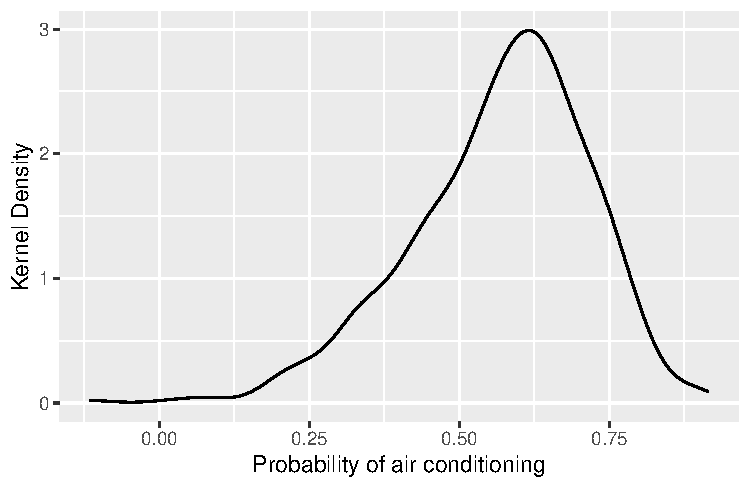
\includegraphics[width=\maxwidth]{figure/unnamed-chunk-10-1} 

}


\end{knitrout}
\end{frame}

\begin{frame}[fragile]\frametitle{Plot of Probability vs.\ Adoption}
\begin{knitrout}\footnotesize
\definecolor{shadecolor}{rgb}{0.969, 0.969, 0.969}\color{fgcolor}\begin{kframe}
\begin{alltt}
\hlcom{## Plot air conditioning vs. probability of air conditioning}
\hlstd{ac_data} \hlopt
  \hlkwd{ggplot}\hlstd{(}\hlkwd{aes}\hlstd{(}\hlkwc{x} \hlstd{= probability_ac_lpm,} \hlkwc{y} \hlstd{= air_conditioning))} \hlopt{+}
  \hlkwd{geom_point}\hlstd{()} \hlopt{+}
  \hlkwd{xlab}\hlstd{(}\hlstr{'Probability of air conditioning'}\hlstd{)} \hlopt{+}
  \hlkwd{ylab}\hlstd{(}\hlstr{'Air conditioning'}\hlstd{)}
\end{alltt}
\end{kframe}
\end{knitrout}
\end{frame}

\begin{frame}[fragile]\frametitle{Plot of Probability vs.\ Adoption}
\begin{knitrout}\footnotesize
\definecolor{shadecolor}{rgb}{0.969, 0.969, 0.969}\color{fgcolor}

{\centering 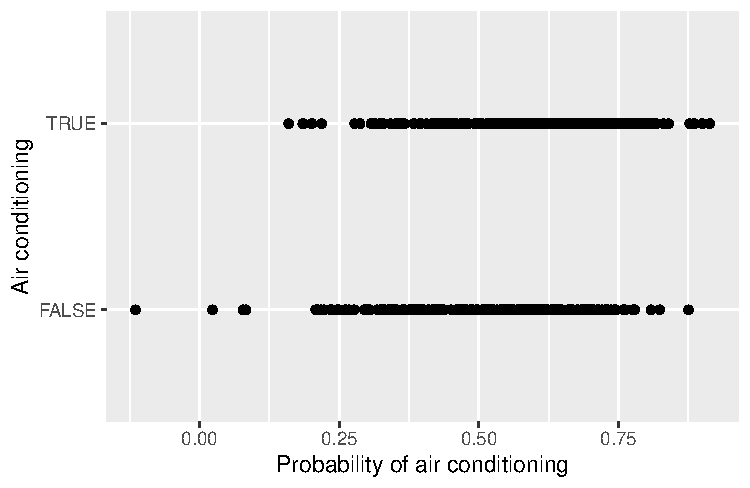
\includegraphics[width=\maxwidth]{figure/unnamed-chunk-12-1} 

}


\end{knitrout}
\end{frame}

\begin{frame}[fragile]\frametitle{Plot of Probability vs.\ Adoption with Bins}
\begin{knitrout}\footnotesize
\definecolor{shadecolor}{rgb}{0.969, 0.969, 0.969}\color{fgcolor}\begin{kframe}
\begin{alltt}
\hlcom{## Plot fraction vs. probability of air conditioning using bins}
\hlstd{ac_data} \hlopt
  \hlkwd{mutate}\hlstd{(}\hlkwc{bin} \hlstd{=} \hlkwd{cut}\hlstd{(probability_ac_lpm,}
                   \hlkwc{breaks} \hlstd{=} \hlkwd{seq}\hlstd{(}\hlopt{-}\hlnum{0.2}\hlstd{,} \hlnum{1}\hlstd{,} \hlnum{0.05}\hlstd{),}
                   \hlkwc{labels} \hlstd{=} \hlnum{1}\hlopt{:}\hlnum{24}\hlstd{))} \hlopt
  \hlkwd{group_by}\hlstd{(bin)} \hlopt
  \hlkwd{summarize}\hlstd{(}\hlkwc{fraction_ac} \hlstd{=} \hlkwd{mean}\hlstd{(air_conditioning),} \hlkwc{.groups} \hlstd{=} \hlstr{'drop'}\hlstd{)} \hlopt
  \hlkwd{mutate}\hlstd{(}\hlkwc{bin} \hlstd{=} \hlkwd{as.numeric}\hlstd{(bin),}
         \hlkwc{bin_mid} \hlstd{=} \hlnum{0.05} \hlopt{*} \hlstd{(bin} \hlopt{-} \hlnum{1}\hlstd{)} \hlopt{+} \hlnum{0.025} \hlopt{-} \hlnum{0.2}\hlstd{)} \hlopt
  \hlkwd{ggplot}\hlstd{(}\hlkwd{aes}\hlstd{(}\hlkwc{x} \hlstd{= bin_mid,} \hlkwc{y} \hlstd{= fraction_ac))} \hlopt{+}
  \hlkwd{geom_point}\hlstd{()} \hlopt{+}
  \hlkwd{xlab}\hlstd{(}\hlstr{'Probability of air conditioning'}\hlstd{)} \hlopt{+}
  \hlkwd{ylab}\hlstd{(}\hlstr{'Fraction with air conditioning'}\hlstd{)}
\end{alltt}
\end{kframe}
\end{knitrout}
\end{frame}

\begin{frame}[fragile]\frametitle{Plot of Probability vs.\ Adoption with Bins}
\begin{knitrout}\footnotesize
\definecolor{shadecolor}{rgb}{0.969, 0.969, 0.969}\color{fgcolor}

{\centering 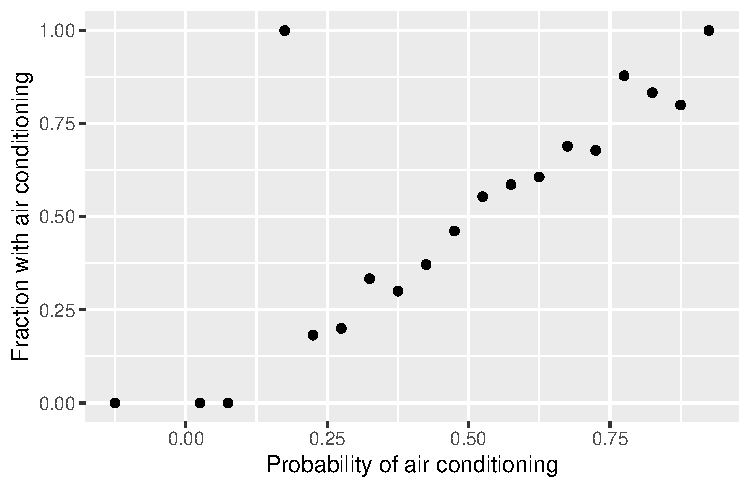
\includegraphics[width=\maxwidth]{figure/unnamed-chunk-14-1} 

}


\end{knitrout}
\end{frame}

\begin{frame}[fragile]\frametitle{Heteroskedastic and Non-Normal Residuals}
    One criticism of a linear probability model is that the error terms are heteroskedastic and not normally distributed
    \begin{itemize}
        \item We can see this issue by calculating the residual for each observation and plotting residuals as a function of fitted probability
    \end{itemize}
\begin{knitrout}\footnotesize
\definecolor{shadecolor}{rgb}{0.969, 0.969, 0.969}\color{fgcolor}\begin{kframe}
\begin{alltt}
\hlcom{## Calculate squared residuals}
\hlstd{ac_data} \hlkwb{<-} \hlstd{ac_data} \hlopt
  \hlkwd{mutate}\hlstd{(}\hlkwc{sq_residual_lpm} \hlstd{= (air_conditioning} \hlopt{-} \hlstd{probability_ac_lpm)}\hlopt{^}\hlnum{2}\hlstd{)}
\hlcom{## Plot squared residual vs. probability of air conditioning}
\hlstd{ac_data} \hlopt
  \hlkwd{ggplot}\hlstd{(}\hlkwd{aes}\hlstd{(}\hlkwc{x} \hlstd{= probability_ac_lpm,} \hlkwc{y} \hlstd{= sq_residual_lpm))} \hlopt{+}
  \hlkwd{geom_point}\hlstd{()} \hlopt{+}
  \hlkwd{xlab}\hlstd{(}\hlstr{'Probability of air conditioning'}\hlstd{)} \hlopt{+}
  \hlkwd{ylab}\hlstd{(}\hlstr{'Squared residual'}\hlstd{)}
\end{alltt}
\end{kframe}
\end{knitrout}
\end{frame}

\begin{frame}[fragile]\frametitle{Heteroskedastic and Non-Normal Residuals}
\begin{knitrout}\footnotesize
\definecolor{shadecolor}{rgb}{0.969, 0.969, 0.969}\color{fgcolor}

{\centering 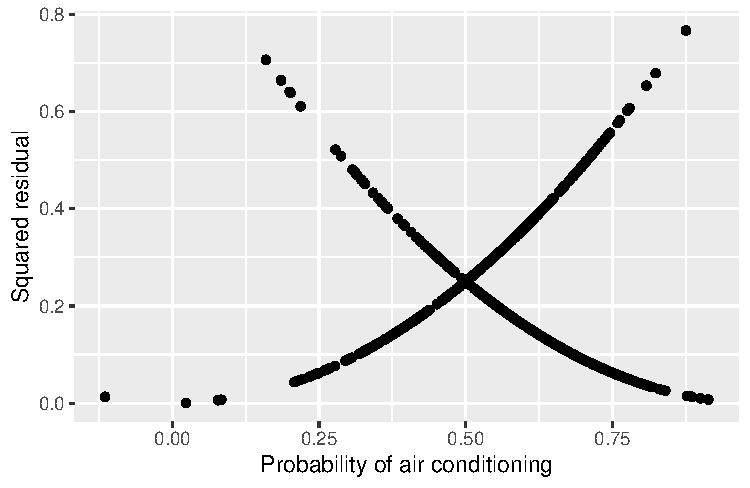
\includegraphics[width=\maxwidth]{figure/unnamed-chunk-16-1} 

}


\end{knitrout}
\end{frame}

\begin{frame}[fragile]\frametitle{Heteroskedastic-Robust Standard Errors}
    \texttt{coeftest()} is a function from the \texttt{lmtest} package to test coefficients and summarize results using an alternate variance-covariance matrix
    \begin{itemize}
        \item \texttt{vcovHC()} is a function from the \texttt{sandwich} package to estimate a heteroskedastic-robust variance-covariance matrix
    \end{itemize}
\begin{knitrout}\footnotesize
\definecolor{shadecolor}{rgb}{0.969, 0.969, 0.969}\color{fgcolor}\begin{kframe}
\begin{alltt}
\hlcom{## Load lmtest and sandwich}
\hlkwd{library}\hlstd{(lmtest)}
\hlkwd{library}\hlstd{(sandwich)}
\hlcom{## Summarize regression results with robust standard errors}
\hlstd{reg_lpm} \hlopt
  \hlkwd{coeftest}\hlstd{(}\hlkwc{vcov} \hlstd{=} \hlkwd{vcovHC}\hlstd{(reg_lpm))}
\end{alltt}
\begin{verbatim}
## 
## t test of coefficients:
## 
##                   Estimate  Std. Error t value  Pr(>|t|)    
## (Intercept)     1.50454126  0.20074465  7.4948 2.408e-13 ***
## cost_system    -0.00067505  0.00033335 -2.0251   0.04331 *  
## cost_operating -0.00346898  0.00046080 -7.5282 1.908e-13 ***
## ---
## Signif. codes:  0 '***' 0.001 '**' 0.01 '*' 0.05 '.' 0.1 ' ' 1
\end{verbatim}
\end{kframe}
\end{knitrout}
\end{frame}

\begin{frame}[fragile]\frametitle{LPM with Heterogeneous Coefficients}
    We have estimated a single ``average'' effect for each price or cost variable
    \begin{itemize}
        \item But in reality, these effects are likely to vary by income
    \end{itemize}
    $$Y_n = \alpha_0 + \alpha_{1n} P_n + \alpha_{2n} C_n + \omega_n$$
    $$\alpha_{1n} = \frac{\alpha_1}{I_n} \quad \text{and} \quad \alpha_{2n} = \frac{\alpha_2}{I_n}$$ \\
    \vspace{2ex}
    Estimate a model using price or cost as a share of income
    $$Y_n = \alpha_0 + \alpha_1 \frac{P_n}{I_n} + \alpha_2 \frac{C_n}{I_n} + \omega_n$$ \\
    \vspace{2ex}
    Use \texttt{I()} around math inside your R formula
\begin{knitrout}\footnotesize
\definecolor{shadecolor}{rgb}{0.969, 0.969, 0.969}\color{fgcolor}\begin{kframe}
\begin{alltt}
\hlcom{## Regress air conditioning on costs divided by income}
\hlstd{reg_lpm_inc} \hlkwb{<-} \hlkwd{lm}\hlstd{(}\hlkwc{formula} \hlstd{= air_conditioning} \hlopt{~} \hlkwd{I}\hlstd{(cost_system} \hlopt{/} \hlstd{income)} \hlopt{+}
                    \hlkwd{I}\hlstd{(cost_operating} \hlopt{/} \hlstd{income),}
                  \hlkwc{data} \hlstd{= ac_data)}
\end{alltt}
\end{kframe}
\end{knitrout}
\end{frame}

\begin{frame}[fragile]\frametitle{LPM with Heterogeneous Coefficients}
\begin{knitrout}\footnotesize
\definecolor{shadecolor}{rgb}{0.969, 0.969, 0.969}\color{fgcolor}\begin{kframe}
\begin{alltt}
\hlcom{## Summarize regression results with robust standard errors}
\hlstd{reg_lpm_inc} \hlopt
  \hlkwd{coeftest}\hlstd{(}\hlkwc{vcov} \hlstd{=} \hlkwd{vcovHC}\hlstd{(reg_lpm_inc))}
\end{alltt}
\begin{verbatim}
## 
## t test of coefficients:
## 
##                           Estimate Std. Error t value  Pr(>|t|)    
## (Intercept)               1.431453   0.060426 23.6893 < 2.2e-16 ***
## I(cost_system/income)    -0.036390   0.007809 -4.6599 3.903e-06 ***
## I(cost_operating/income) -0.176198   0.020526 -8.5842 < 2.2e-16 ***
## ---
## Signif. codes:  0 '***' 0.001 '**' 0.01 '*' 0.05 '.' 0.1 ' ' 1
\end{verbatim}
\end{kframe}
\end{knitrout}
\end{frame}

\begin{frame}[fragile]\frametitle{Interpreting Heterogeneous Coefficients}
\begin{knitrout}\footnotesize
\definecolor{shadecolor}{rgb}{0.969, 0.969, 0.969}\color{fgcolor}\begin{kframe}
\begin{alltt}
\hlcom{## Display regression coefficients}
\hlkwd{coef}\hlstd{(reg_lpm_inc)}
\end{alltt}
\begin{verbatim}
##              (Intercept)    I(cost_system/income) 
##               1.43145289              -0.03638958 
## I(cost_operating/income) 
##              -0.17619786
\end{verbatim}
\end{kframe}
\end{knitrout}
    \vspace{2ex}
    How do we interpret these coefficients?
    \begin{itemize}
        \item An additional 0.1 percentage point of purchase price as a share of income decreases the probability of purchase by 3.64 percentage points
        \item An additional 0.1 percentage point of annual operating cost as a share of decreases the probability of purchase by 17.62 percentage points
    \end{itemize}
\end{frame}

\begin{frame}[fragile]\frametitle{Kernel Density of Income}
\begin{knitrout}\footnotesize
\definecolor{shadecolor}{rgb}{0.969, 0.969, 0.969}\color{fgcolor}\begin{kframe}
\begin{alltt}
\hlcom{## Plot kernel density of income}
\hlstd{ac_data} \hlopt
  \hlkwd{ggplot}\hlstd{(}\hlkwd{aes}\hlstd{(}\hlkwc{x} \hlstd{= income))} \hlopt{+}
  \hlkwd{geom_density}\hlstd{()} \hlopt{+}
  \hlkwd{xlab}\hlstd{(}\hlstr{'Income'}\hlstd{)} \hlopt{+}
  \hlkwd{ylab}\hlstd{(}\hlstr{'Kernel density'}\hlstd{)}
\end{alltt}
\end{kframe}
\end{knitrout}
\end{frame}

\begin{frame}[fragile]\frametitle{Kernel Density of Income}
\begin{knitrout}\footnotesize
\definecolor{shadecolor}{rgb}{0.969, 0.969, 0.969}\color{fgcolor}

{\centering 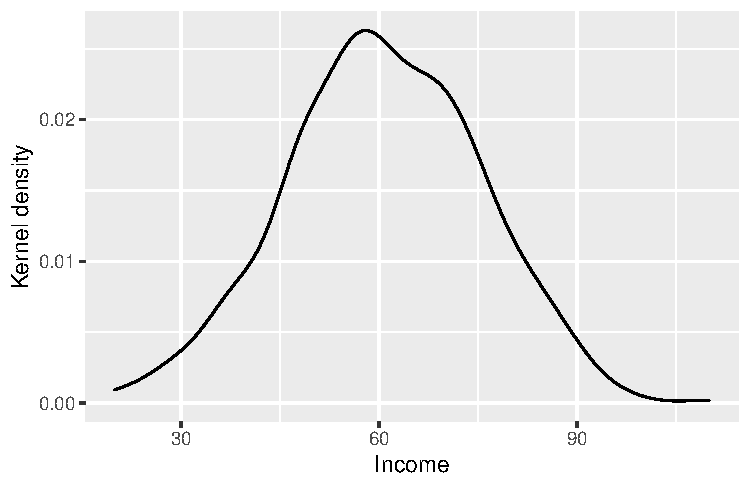
\includegraphics[width=\maxwidth]{figure/unnamed-chunk-22-1} 

}


\end{knitrout}
\end{frame}

\begin{frame}[fragile]\frametitle{Marginal Effects Depending on Income}
    What are the marginal effects at \$30,000 income? \$60,000? \$90,000?
    $$\alpha_{1n} = \frac{\alpha_1}{I_n} \quad \text{and} \quad \alpha_{2n} = \frac{\alpha_2}{I_n}$$
\begin{knitrout}\footnotesize
\definecolor{shadecolor}{rgb}{0.969, 0.969, 0.969}\color{fgcolor}\begin{kframe}
\begin{alltt}
\hlcom{## Calculate marginal effects of costs when income == 30}
\hlkwd{coef}\hlstd{(reg_lpm_inc)[}\hlnum{2}\hlopt{:}\hlnum{3}\hlstd{]} \hlopt{/} \hlnum{30}
\end{alltt}
\begin{verbatim}
##    I(cost_system/income) I(cost_operating/income) 
##             -0.001212986             -0.005873262
\end{verbatim}
\begin{alltt}
\hlcom{## Calculate marginal effects of costs when income == 60}
\hlkwd{coef}\hlstd{(reg_lpm_inc)[}\hlnum{2}\hlopt{:}\hlnum{3}\hlstd{]} \hlopt{/} \hlnum{60}
\end{alltt}
\begin{verbatim}
##    I(cost_system/income) I(cost_operating/income) 
##            -0.0006064931            -0.0029366309
\end{verbatim}
\begin{alltt}
\hlcom{## Calculate marginal effects of costs when income == 90}
\hlkwd{coef}\hlstd{(reg_lpm_inc)[}\hlnum{2}\hlopt{:}\hlnum{3}\hlstd{]} \hlopt{/} \hlnum{90}
\end{alltt}
\begin{verbatim}
##    I(cost_system/income) I(cost_operating/income) 
##            -0.0004043287            -0.0019577540
\end{verbatim}
\end{kframe}
\end{knitrout}
\end{frame}

\begin{frame}[fragile]\frametitle{LPM with Residents as an Explanatory Variable}
    We can include other attributes of households in the linear probability model
    \begin{itemize}
        \item Number of residents, size of apartment, etc.
    \end{itemize}
\begin{knitrout}\footnotesize
\definecolor{shadecolor}{rgb}{0.969, 0.969, 0.969}\color{fgcolor}\begin{kframe}
\begin{alltt}
\hlcom{## Regress air conditioning on scaled costs and number of residents}
\hlstd{reg_lpm_res} \hlkwb{<-} \hlkwd{lm}\hlstd{(}\hlkwc{formula} \hlstd{= air_conditioning} \hlopt{~} \hlkwd{I}\hlstd{(cost_system} \hlopt{/} \hlstd{income)} \hlopt{+}
                    \hlkwd{I}\hlstd{(cost_operating} \hlopt{/} \hlstd{income)} \hlopt{+} \hlstd{residents,}
                  \hlkwc{data} \hlstd{= ac_data)}
\hlcom{## Summarize regression results with robust standard errors}
\hlstd{reg_lpm_res} \hlopt
  \hlkwd{coeftest}\hlstd{(}\hlkwc{vcov} \hlstd{=} \hlkwd{vcovHC}\hlstd{(reg_lpm_res))}
\end{alltt}
\begin{verbatim}
## 
## t test of coefficients:
## 
##                            Estimate Std. Error  t value  Pr(>|t|)    
## (Intercept)               0.8592807  0.0719445  11.9437 < 2.2e-16 ***
## I(cost_system/income)    -0.0357436  0.0074886  -4.7731 2.285e-06 ***
## I(cost_operating/income) -0.1841899  0.0176557 -10.4323 < 2.2e-16 ***
## residents                 0.3430781  0.0159653  21.4890 < 2.2e-16 ***
## ---
## Signif. codes:  0 '***' 0.001 '**' 0.01 '*' 0.05 '.' 0.1 ' ' 1
\end{verbatim}
\end{kframe}
\end{knitrout}
\end{frame}

\end{document}
